\documentclass[t, 10pt]{beamer}
%%\documentclass[t,handout]{beamer}

\usepackage{graphicx}
\usepackage{epsfig}
\usepackage{psfrag}
\usepackage[english]{babel}
\usepackage{color}
%Mathematics packages
\usepackage{amsmath}
\usepackage{mathrsfs}
\usepackage{amsfonts}

\usepackage{enumerate}


\graphicspath{{./images/}} % Figures path - used in graphicx

\selectcolormodel{cmyk}

\mode<presentation>

%THEMES - Please refer to these chapters in the beamer documentation.
% Presentation themes : Chapter 15
% Color themes : Chapter 17
% Font themes : Chapter 18


\usetheme{Pittsburgh}
\usecolortheme{orchid}
\usefonttheme{default}

%---------------------------Title frame definition------------------------------------- 

\title{Managed Control of Composite Cloud Systems}
\author [Chris]{Christopher C. Lamb, Pramod A. Jamkhedkar, Gregory L. Heileman, and Chaouki T. Abdallah}
\institute[University of New Mexico]{
\inst {}Department of Electrical and Computer Engineering\\
University of New Mexico}
\date{June 10, 2011}
\titlegraphic{
\begin{figure} 

\includegraphics[width = 7cm]{UNM}
\end{figure}}

% Delete this, if you do not want the table of contents to pop up at
% the beginning of each subsection:
%\AtBeginSubsection[]
%{
%  \begin{frame}<beamer>
%    \frametitle{Outline}
%     \tableofcontents[currentsection,currentsubsection]
%  \end{frame}
%}

\begin{document}

\begin{frame}
\titlepage
\end{frame}

% This command will make the logo appear on all frames excluding the title frame.
\logo {
\includegraphics[width = 2.5cm]{UNM}}

\begin{frame}
\frametitle{Outline}
\tableofcontents 
\end{frame}

\section{UNM Informatics}
\begin{frame}
\frametitle{Areas of Study}

Our group:
\begin{itemize}
\item \textit{UNM Informatics} \\
 Information security, theory, and architectures; this work is specific to information security 
\item \textit{Usage Management} \\
Control of how an artifact is used, covering everything \textit{after} access as well as controlling access itself
\end{itemize}
%\pause

\textit{Motivation}: We believe people should have control over their own information.  Or past motivation for DRM work was to provide content control to content creators.  Doing so provides incentive for innovation, and improves quality of life for individuals and society as a whole over time.  We believe Usage Management provides the same benefits, and should be unobtrusive.
\newline
\newline
%\pause
This motivation holds in this domain as well.
\end{frame}

\section{Usage Management and Cloud Systems}
\begin{frame}
\frametitle{Why is this important?}
Utility computing will certainly be the most pervasive future computing model \\
%\pause
\begin{itemize}
\item \textit{Mainframes won!}
%\pause
\begin{itemize}
\item Well, end devices are powerful
\item Cloud computing pervasive for \textit{convenience}, not \textit{technical necessity}.
\item \textit{Still resembles centralized models of the past}
\end{itemize}
%\pause
\item \textit{People should control what they own}
\begin{itemize}
\item Access
\item Retention
\item Distribution
\end{itemize}
%\pause 
\item \textit{Organizations should control what they pay for}
\begin{itemize}
\item Systems
\item Data
\item Records
\end{itemize}
\end{itemize}
\end{frame}

\begin{frame}
\frametitle{Problems}
So this is what we would like to see, but problems abound
\begin{itemize}
\item \textit{Scalability, performance, usability, infrastructural support...}
\end{itemize}
%\pause
Started examining automation and ability to combine service level agreements (SLAs)
\begin{itemize}
\item \textit{Automation} \\
How we can automate control and enforcement
\item \textit{Combine} \\
How we can combine multiple SLAs into single SLAs
\end{itemize}
%\pause

Surprisingly difficult...
\begin{itemize}
\item \textit{NP-Complete} \\
Simple generalized SLAs are equivalent to \textit{SAT}
\item \textit{Multiple Providers} \\
Difficult constant factors related to latency, etc.
\end{itemize}
 
\end{frame}

\section{Example Systems}
\begin{frame}
\frametitle{Single Provider, Feedback}

\begin{figure}
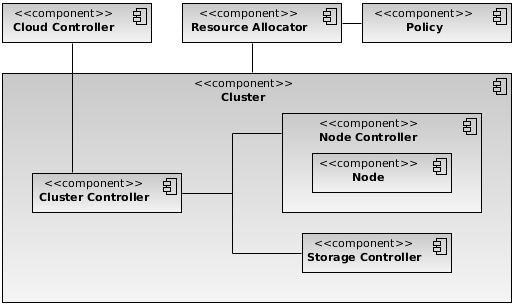
\includegraphics[width = 8cm]{Single-QoS}
\end{figure}

Things we care about: \\
\begin{itemize}
\item \textit{Performance, Accessibility, Controllability}
\end{itemize}

\end{frame}

\begin{frame}
\frametitle{Single Provider, Feedback}

\begin{itemize}
\item \textit{Cloud Controller} Provides an initial interface to administrative users to control the cloud.
\item \textit{Cluster Controller} Managed by the cloud controller, the cluster controller manages the resources of a single cluster.
\item \textit{Storage Controller} Provides storage of system images and for other general storage needs.
\item \textit{Node Controller} Responsible for allocating, delivering, and managing individual compute nodes upon which client software runs.
\item \textit{Node} The compute node delivering services to end users and managed by the cluster's control infrastructure.
\item \textit{Policy} Quality of service terms the cloud provider has agreed to honor for the cloud customer.
\item \textit{Resource Allocator} The component responsible for real-time tuning of the cloud system to maintain defined quality of service.
\end{itemize}

\end{frame}

\begin{frame}
\frametitle{Single Provider, Feedback}
The \textit{resource controller} tunes the \textit{cluster} based on obligations defined within the \textit{policy}. \\

\begin{figure}
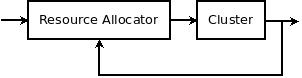
\includegraphics[width = 5cm]{feedback}
\end{figure}

Multiple possible control loops:
\begin{itemize}
\item \textit{Physical Loop} \\
Controls lower level server or rack specific attributes like cooling or power consumption
\item \textit{Service Loop} \\
Controls responses for the provider as a whole according to contractual obligations
\end{itemize}

Watch out for timing problems, inflexibility, intractable traceability

\end{frame}

\begin{frame}
\frametitle{Single Provider, Feedback with UM}

\begin{figure}
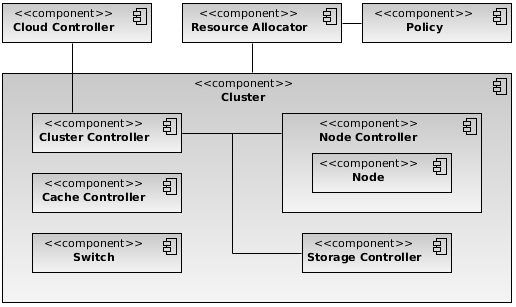
\includegraphics[width = 8cm]{Single-UM}
\end{figure}

New things we care about: \\
\begin{itemize}
\item \textit{Accessibility}
\end{itemize}

\end{frame}

\begin{frame}
\frametitle{Single Provider, Feedback with UM}

\begin{itemize}
\item \textit{Cache Controllers} Streaming network data, specifically media-centric streams, can and are cached by strategically located cache systems.  In order to control the read access of network data, we must be able to exercise explicit control over any caching systems in our infrastructure.
\item \textit{Switch} Really any kind of hardware that controls the delivery of network data.  This component includes switches and routers primarily.  In order to control how data is accessed we must be able to control the locations to which it is delivered.
\end{itemize}

\end{frame}

\begin{frame}
\frametitle{Single Provider, Feedback with UM}
We have also added a new relationship to enable control over the \textit{Cloud Controller}.  To ensure that we can control where data is at any given time, we must also be able to control the geographic areas from which data is generated, especially if the virtual compute cloud spans national boundaries.
\newline
\newline
We also must be able to control where specifically the data resides; ergo we must have control over caches and switches
\newline
\newline
As the system is growing, we have:
\begin{itemize}
\item \textit{More Complexity} \\
New relationships and elements
\item \textit{Growth is Linear} \\
We do control new items, but growth is not geometric
\end{itemize}

\end{frame}

\begin{frame}
\frametitle{Multiple Providers}

\begin{figure}
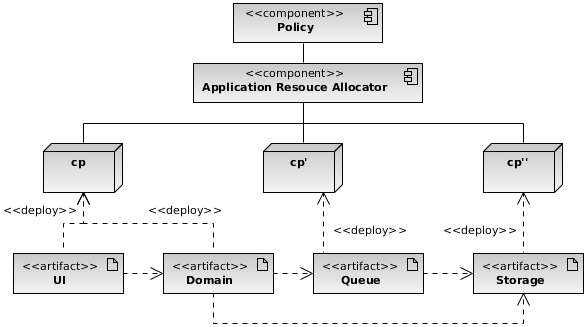
\includegraphics[width = 8cm]{Multiple}
\end{figure}

New Concepts:
\begin{itemize}
\item \textit{Provider Service Differentiation} \\
Multiple providers involved offering different services
\item \textit{Control Perspectives} \\
We now include a client-centric perspective
\end{itemize}

\end{frame}

\begin{frame}
\frametitle{Multiple Providers}
We now have three different cloud providers
\begin{itemize}
\item $ cp $ \\
...provides hosting for the \textit{User Interface} and \textit{Domain} layers 
\item $ cp' $ \\
...provides queuing services to the application
\item $ cp'' $ \\
...provides data storage
 \end{itemize}
 
Each cloud provider contains the same elements contained by the providers in the previous sections, including a \textit{Resource Allocator} specific to that cloud provider
\newline
\newline
Application control problematic...\\\
...cloud control complexity is linear, \textit{Application} control is exponential in number of involved systems
 
\end{frame}

\section{Conclusions and Future Work}
\begin{frame}
\frametitle{Conclusions and Future Work}
Conclusions include...
\begin{itemize}
\item Difficult restrictions on control
\item Possibly brittle
\item Difficult to predict and time sensitive
\item Becomes very complex from cloud client perspective
\end{itemize}
Future work involves more rigorous analysis of multiple provider complexity and implementation and validation of initial control models
\end{frame}

%\bibliographystyle{plain}
%\bibliography{drm}

\end{document}

